\section{实验部分 - FTPL}

\subsection{基本结构}

本实验主要分为两部分:
\begin{itemize}
    \item FTPL.py: 主程序,实现 FTPL 算法
    \item utils.py: 工具函数,负责处理数据(离散化)
\end{itemize}

\subsection{utils.py}

\subsubsection{离散化价格空间}

首先需要离散化价格空间,将连续的价格区间 $[0, 1]$ 离散化为点集。

\begin{itemize}
    \item 设置 $Z_i$ 点作为分割区间的依据:$Z_i = \epsilon(1+\epsilon)^i,\quad i \in \left\{ 0, 1, \ldots, \left\lceil \log_{1+\epsilon} \frac{1}{\epsilon} \right\rceil \right\}$
    \item 根据 $Z_i$ 点,构建离散化价格空间 $W$:
    \begin{itemize}
        \item 区间 $W_i$ 是范围为 $[Z_{i-1},Z_{i+1})$ 的均匀离散化,间隔为 $Z_{i-1}\cdot \cfrac{\epsilon}{m}$
        \item 更具体的, $W_i = \{Z_{i-1} + Z_{i-1}\cdot \cfrac{\epsilon k}{m}\mid k\in \{1,2,\dots,\lceil(2+\epsilon)m\rceil\}\}$
        \item 将这些区间并起来,我们就得到了离散化的价格空间 $W = \bigcup_{i=1}^{\lceil \log_{1+\epsilon} \frac{1}{\epsilon} \rceil} W_i$
    \end{itemize}
\end{itemize}

现在我们可以初步构建离散的价格曲线空间 $\overline{\mathcal{P}}$,其中每个价格曲线 $p$ 是一个函数,定义为 $p: [N] \to W$。这个价格曲线空间的复杂度仍然有些高,因此我们需要更进一步,将数量空间离散化

\subsubsection{离散化物品数量空间}

物品数量空间为 $[0, N]$,虽然其已经是离散的,但为了进一步减少其复杂度,我们将其离散化为更小的点集 $N_D$。

\begin{itemize}
    \item 定义阈值 $\lfloor \cfrac{2Jm}{\epsilon^2}\rfloor$,我们只离散化高于这个阈值的数量
    \item 设置 $Y_i$ 点作为分割区间的依据:$Y_i = \lfloor\cfrac{2Jm}{\epsilon^2}(1+\epsilon^2)^i\rfloor,\quad i=0,\ldots, \lceil\log_{1+\epsilon^2} \frac{N\epsilon^2}{2Jm}\rceil$
    \item 对于每个 $Y_i$,我们在区间 $[Y_i, Y_{i+1})$ 上均匀离散化,间隔为 $Y_i\cdot \cfrac{\epsilon^2}{2Jm}$,得到点集 $Q_i$
    \item 将这些区间并起来,得到:$Q = \bigcup_{i=0}^{\lceil\log_{1+\epsilon^2} \frac{N\epsilon^2}{2Jm}\rceil} Q_i$
    \item 最后补上阈值及之下的点集,得到 $N_D = \{1, 2, \ldots, \lfloor \cfrac{2Jm}{\epsilon^2} \rfloor\} \cup Q$
\end{itemize}

\subsubsection{构建阶梯价格曲线}

现在我们可以构建阶梯价格曲线集合 $\overline{\mathcal{P}}$,其中每个价格曲线 $p$ 是一个函数,定义为 $p: N_D \to W$。

\begin{itemize}
    \item 由于可能的价格曲线非常多,这里使用了采样数量 `sample_num' 来作为随机采样的数量
    \item 每轮采样,先从 1 到 $m$ 中随机选择一个整数 $k$,作为阶梯的数量
    \item 如果 $k = 1$,那么函数是常数函数,直接从价格空间中随机选择一个价格,构建从 $[N]$ 到该价格的函数
    \item 如果 $k > 1$,则要构建一个多段的阶梯函数,这个阶梯函数有 $k-1$ 个跳变点和 $k$ 个价格点
    \begin{itemize}
        \item 首先选择 $k-1$ 个跳变点 $j_1,j_2,\dots ,j_{k-1}$,这些点从数量空间 $N_D$ 中随机采样,排除 0 和 $N$
        \item 然后选择 $k$ 个价格点 $p_1,p_2,\dots ,p_k$,这些点从价格空间 $W$ 中随机采样
        \item 最后将这些价格点和跳变点组合成一个阶梯函数得到价格曲线 $p$ 如下:
        \[
            p(n) = 
            \begin{cases}
                p_1 & \text{if } 0 \leq n < j_1 \\
                p_2 & \text{if } j_1 \leq n < j_2 \\
                \vdots & \vdots \\
                p_k & \text{if } j_{k-1} \leq n \leq N \\
            \end{cases}
        \]
    \end{itemize}
    \item 这样就得到了一个阶梯价格曲线集合 $\overline{\mathcal{P}}$
\end{itemize}

\subsection{FTPL.py}

\subsubsection{基本参数}

\begin{itemize}
    \item $N$: 物品数量(默认 100)
    \item $m$: 买家类型数量,同时也是阶梯函数的最大阶数(默认 20)
    \item $J$: 收益递减常数(默认 2)
    \item $T$: 总回合数(默认 20)
    \item $\epsilon$:近似精度参数(默认 0.08)
    \item $\theta$: 随机噪声参数(默认 1)
    \item $sample\_num$: 每轮采样的价格曲线数量(默认 20000)
    \item $valuation$: 买家估值函数,定义为 $v_i(n) = V - b \cdot e^{-a \cdot n}$
    \begin{itemize}
        \item $V$: 基础价值,随着买家类型变化(例如 $0.2 + \frac{buyer\_type}{T}$)
        \item $a$: 递减率,随着买家类型变化(例如 $0.1 + buyer\_type \cdot 0.01$)
        \item $b$: 价格影响系数,随着买家类型变化(例如 $0.2 + buyer\_type \cdot 0.01$)
    \end{itemize}
\end{itemize}

\subsubsection{FTPL 算法}

FTPL 部分的步骤如下:

\begin{itemize}
    \item 初始化参数和变量,包括价格曲线集合 $\overline{\mathcal{P}}$ 和以及每个价格曲线的收益
    \item 在每轮中,执行如下步骤:
    \begin{enumerate}
        \item 卖家根据策略选择一个价格曲线 $p \in \overline{\mathcal{P}}$
        \item 一个对抗性策略选择买家类型 $t \in [m]$,以降低卖家的收益
        \item 买家根据自己类型进行最优购买
        \item 计算卖家的收益 $r_t(p)$,同时更新并记录所有信息
    \end{enumerate}
    \item 重复上述步骤直到达到总回合数 $T$,最终会将记录的信息可视化展示
\end{itemize}

\paragraph{卖家定价}

\begin{itemize}
    \item 在开始总买卖之前,先对每个价格曲线 $p \in \overline{\mathcal{P}}$ 从分布 $\theta e^{-\theta x}$ 中采样一个噪声 $\theta_p$
    \item 第 $t$ 轮中,计算每条价格曲线 $p$ 的历史收益(含噪声) $r(p) = \sum_{i=1}^{t-1} r_i(p) + \theta_p$
    \item 选择收益最大的价格曲线 $p_t = \arg\max_{p \in \overline{\mathcal{P}}} r(p)$
\end{itemize}

\paragraph{买家最优购买}
\begin{itemize}
    \item 买家类型 $i$ 根据价格曲线 $p_t$ 和估值函数 $v_i(n)$ 进行购买决策
    \item 对于每种购买数量,计算效用函数 $u_i(n) = v_i(n) - p_t(n)$
    \item 如果所有效用不大于 0,则不购买,否则选择效用最大的购买量 $n_{i_t,p_t} = \arg\max_{n} u_i(n)$
    \item 如果存在多个效用相等的最大值,则选择最大的 $n$
\end{itemize}

\paragraph{对抗性生成买家类型}

\begin{itemize}
    \item 对抗性策略会选择一个买家类型 $i_t$,使得卖家的收益最小化
    \item 具体来说,对于每个买家类型 $i$,由最优购买策略计算当前价格曲线下的购买数量 $n_{i,p_t}$
    \item 选择使得卖家收益 $r_t(p_t)$ 最小的买家类型 $i_t = \arg\min_{i} p(n_{i_t,p_t})$
\end{itemize}

\paragraph{收益计算与更新}

\begin{itemize}
    \item 根据买家购买数量 $n_{i_t,p_t}$,来分类计算卖家的收益
    \item 如果 $n_{i_t,p_t} > 0$,则对所有价格曲线 $p\in \overline{\mathcal{P}}$,其本轮收益为 $r_t(p) = p(n_{i_t,p})$
    \item 如果 $n_{i_t,p_t} = 0$,则:
    \begin{itemize}
        \item 将所有在当前价格曲线下购买数量为 0 的买家记为集合 $S_t^c$
        \item 对所有价格曲线 $p\in \overline{\mathcal{P}}$,其本轮收益为 $r_t(p) = \sum_{i \in S_t^c} p(n_{i,p})$
    \end{itemize}
    \item 计算遗憾值:$R_t = \max_{p \in \overline{\mathcal{P}}} \sum_{t=1}^T p(n_{i_t},p) - \sum_{t=1}^T p_t(n_{i_t},p_t)$,即卖家在最好的价格曲线下的总收益减去实际的总收益
    \item 记录历史收益、遗憾值以及买家类型等信息
\end{itemize}

\subsection{结果分析}

\begin{figure}[H]
    \centering
    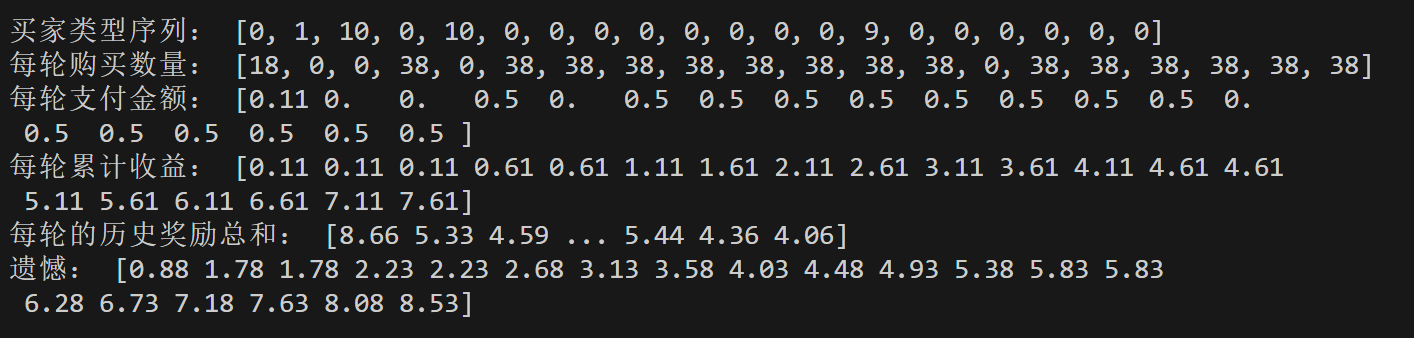
\includegraphics[width=0.92\textwidth]{figures/FTPL_1}
    \caption{FTPL 终端输出}
\end{figure}

这里展示了 FTPL 算法的终端输出结果,包括每轮的收益、遗憾值以及买家类型等信息,具体可视化结果在后面的图表中。

\begin{figure}[H]
    \centering
    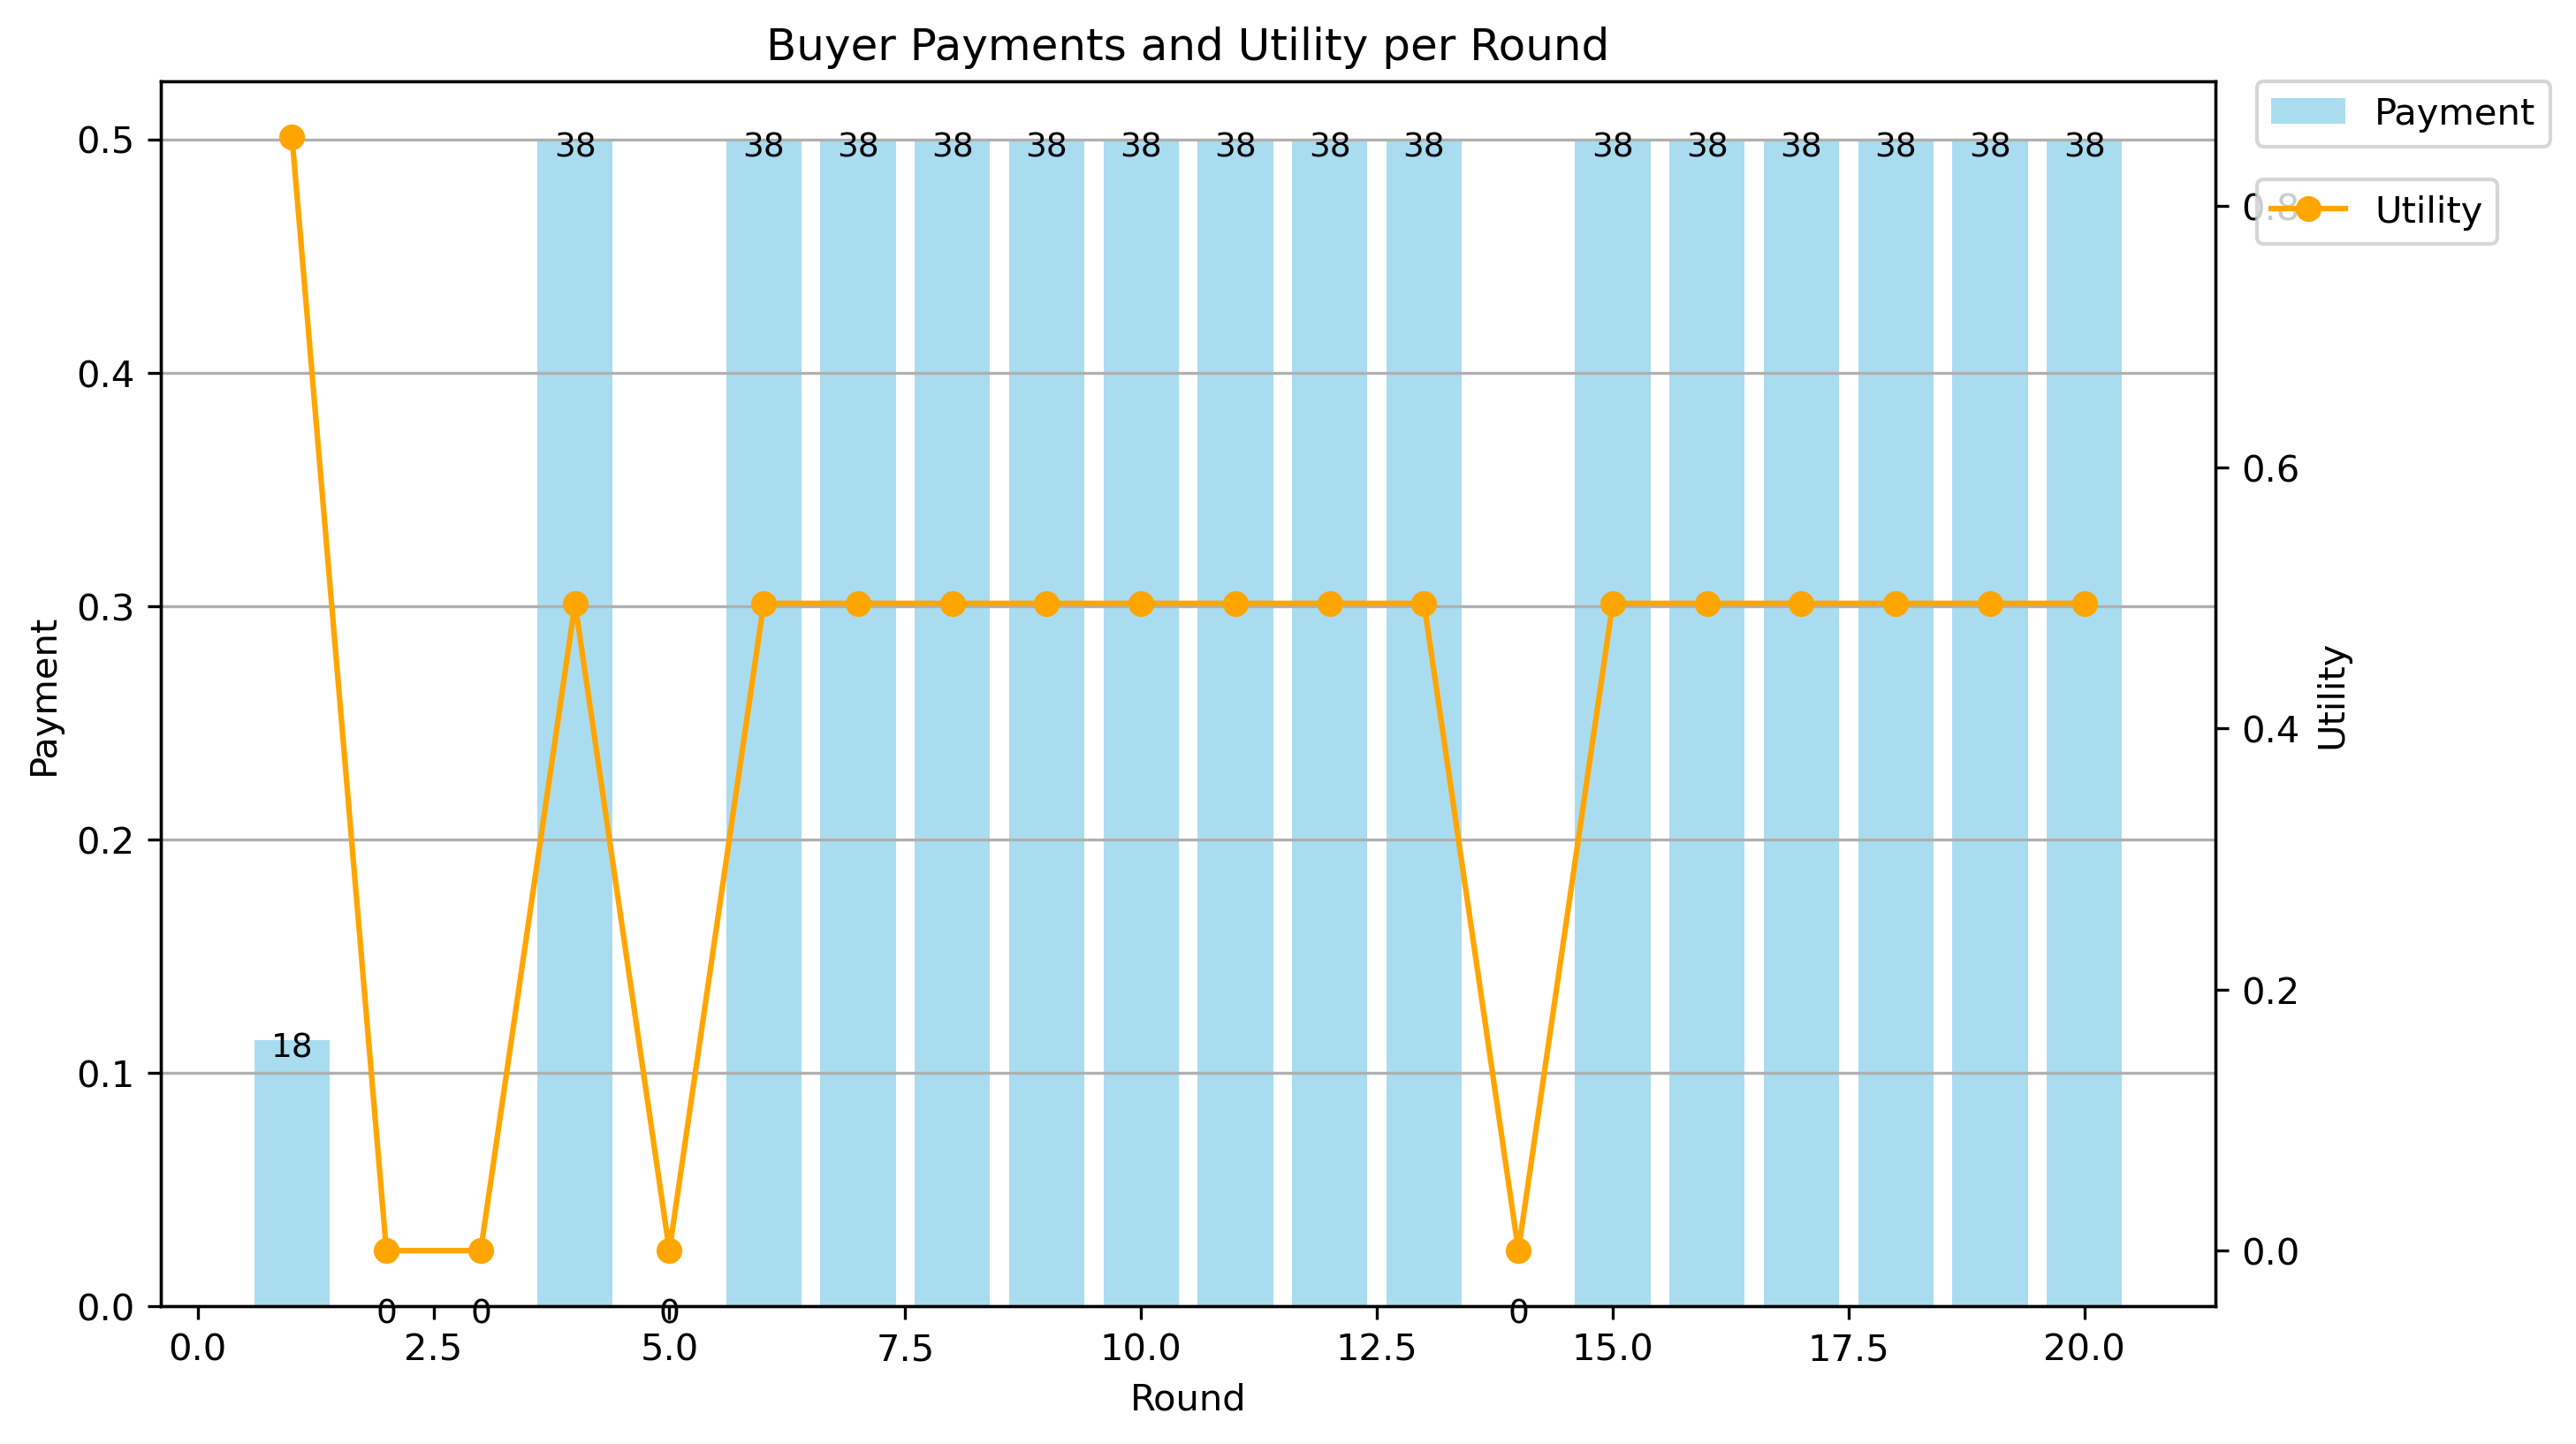
\includegraphics[width=0.92\textwidth]{figures/FTPL_buyer_payments}
    \caption{FTPL 买家支付及效益情况}
\end{figure}

柱状图展示了每轮中卖家的支付情况,左侧坐标为买家支付的金额,右侧坐标为买家的效用值。柱状图上方的数字为购买的数量。叠加的折线图展示了买家的效用情况。

\begin{figure}[H]
    \centering
    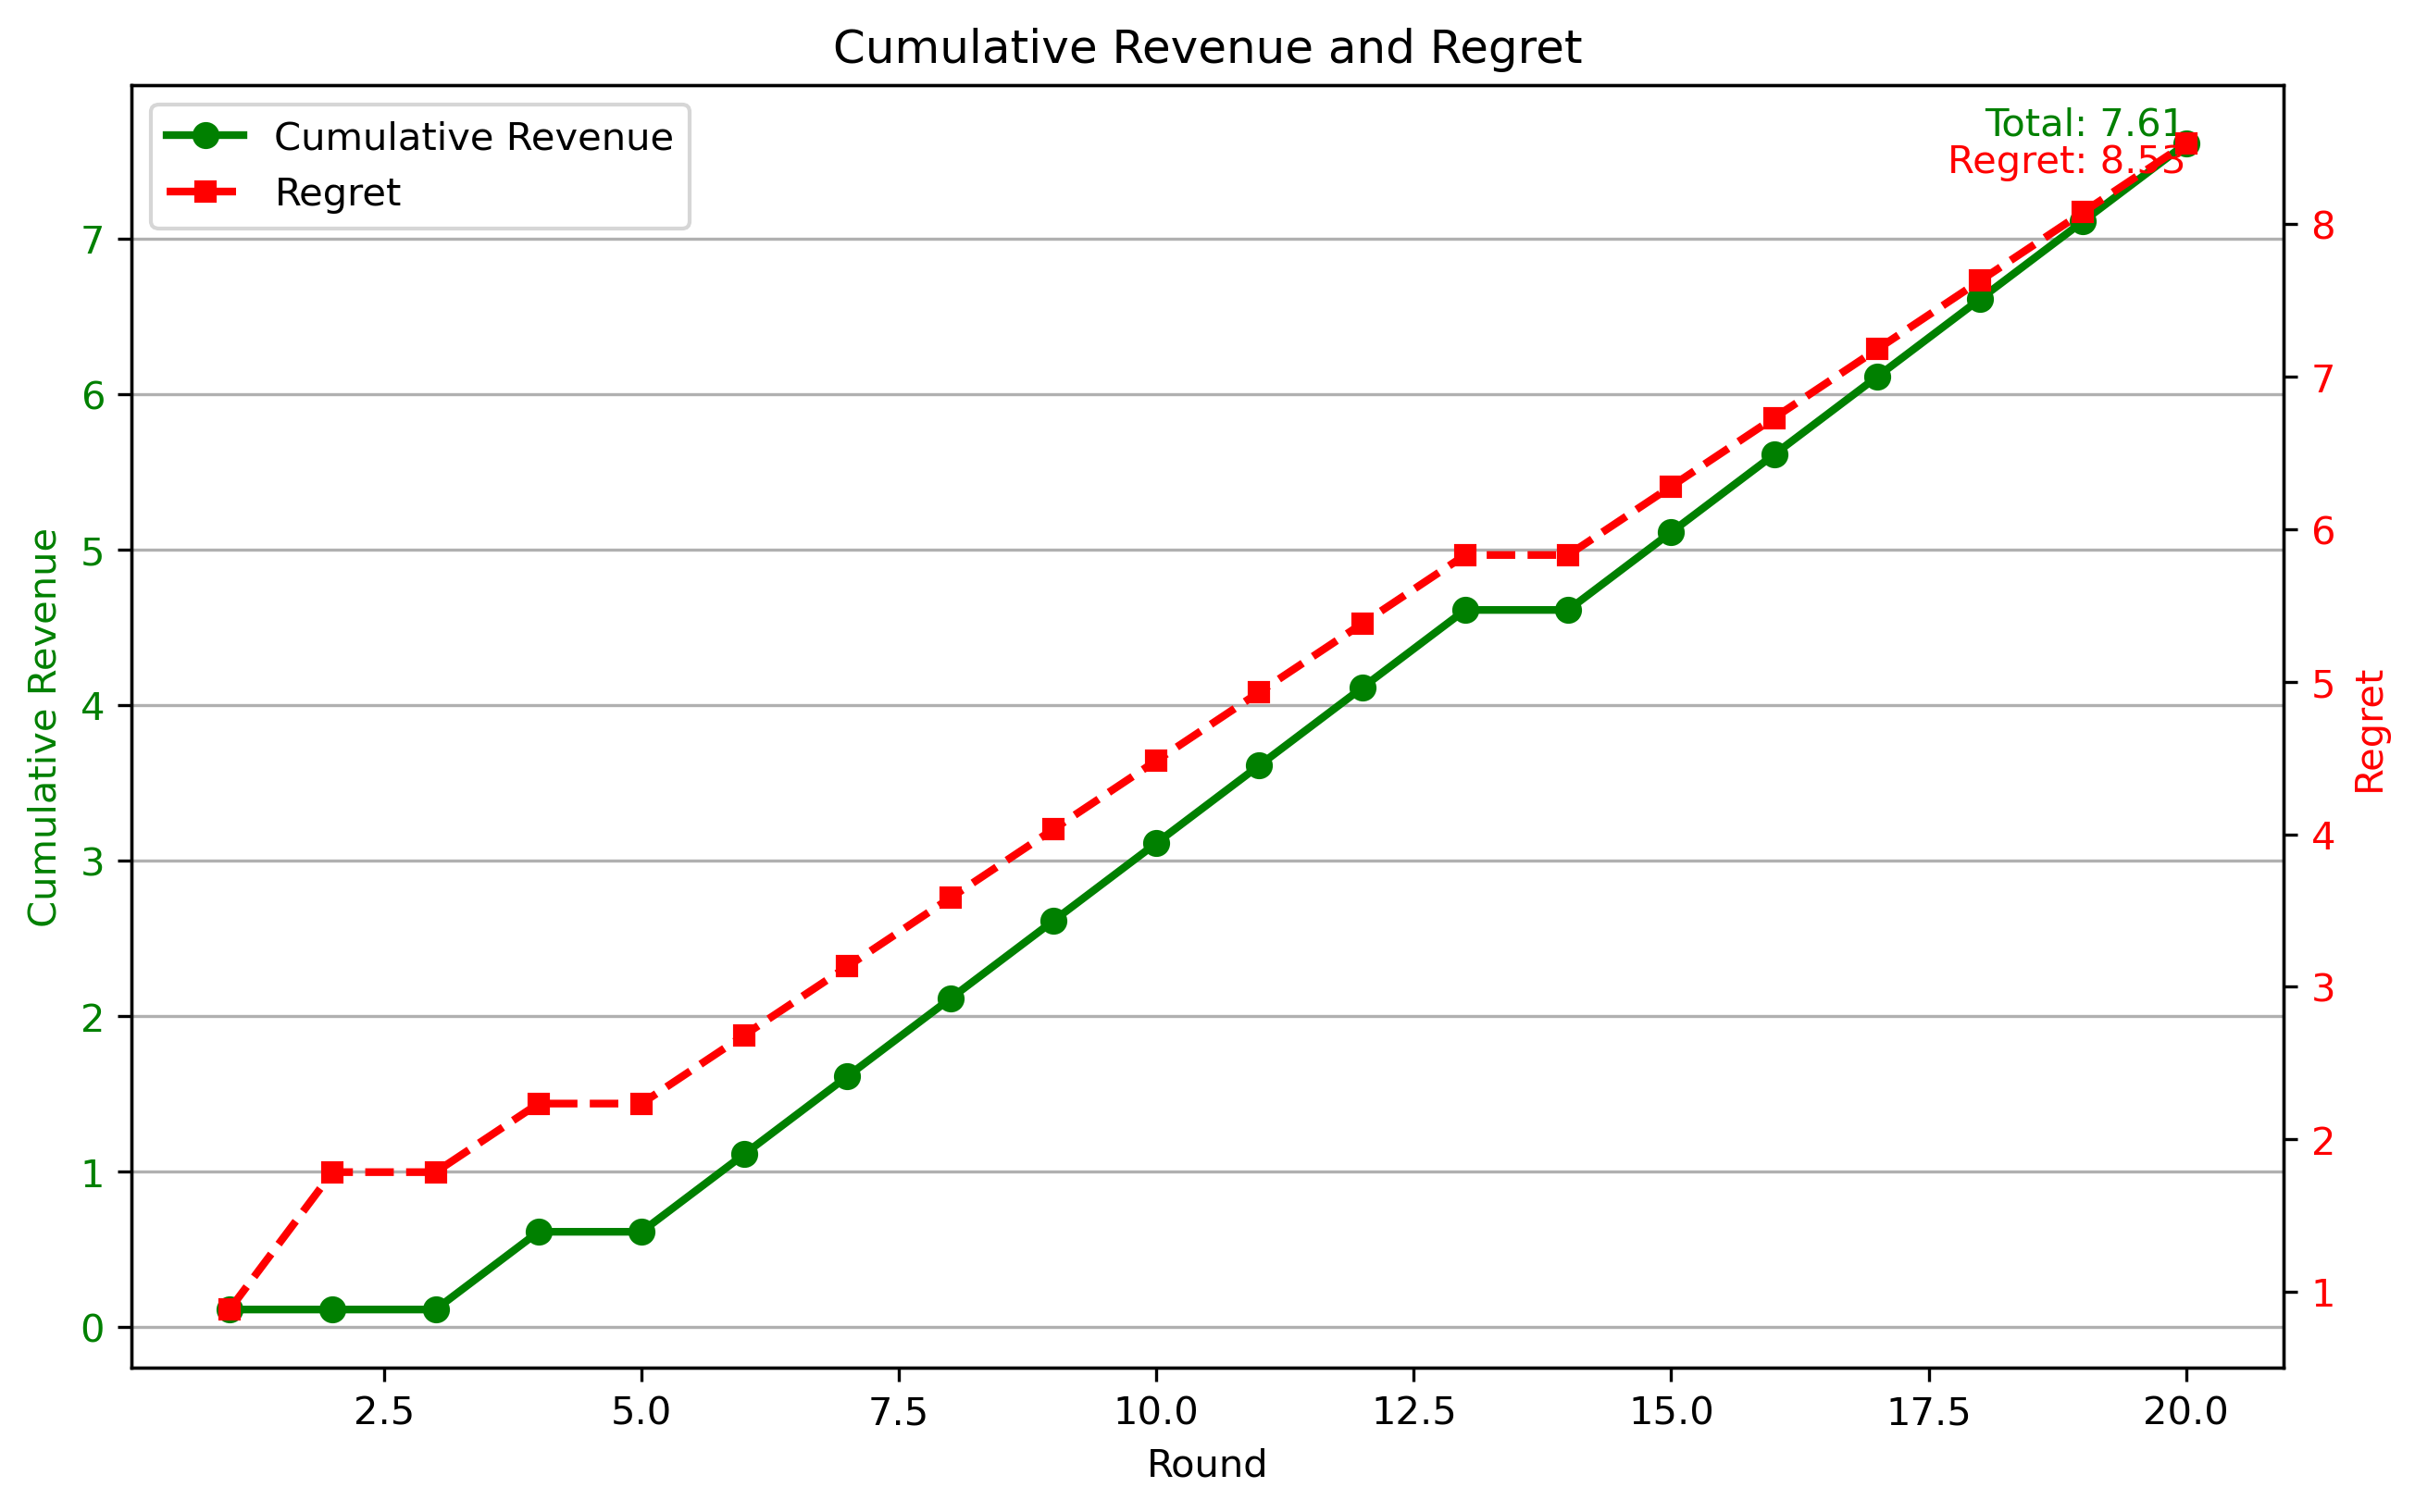
\includegraphics[width=0.92\textwidth]{figures/FTPL_cumulative_revenue}
    \caption{FTPL 累计收益及遗憾}
\end{figure}

绿色实现表示卖家的累计收益,红色虚线表示卖家的遗憾值。随着轮次的增加,卖家的累计收益和遗憾值逐渐增加。

\begin{figure}[H]
    \centering
    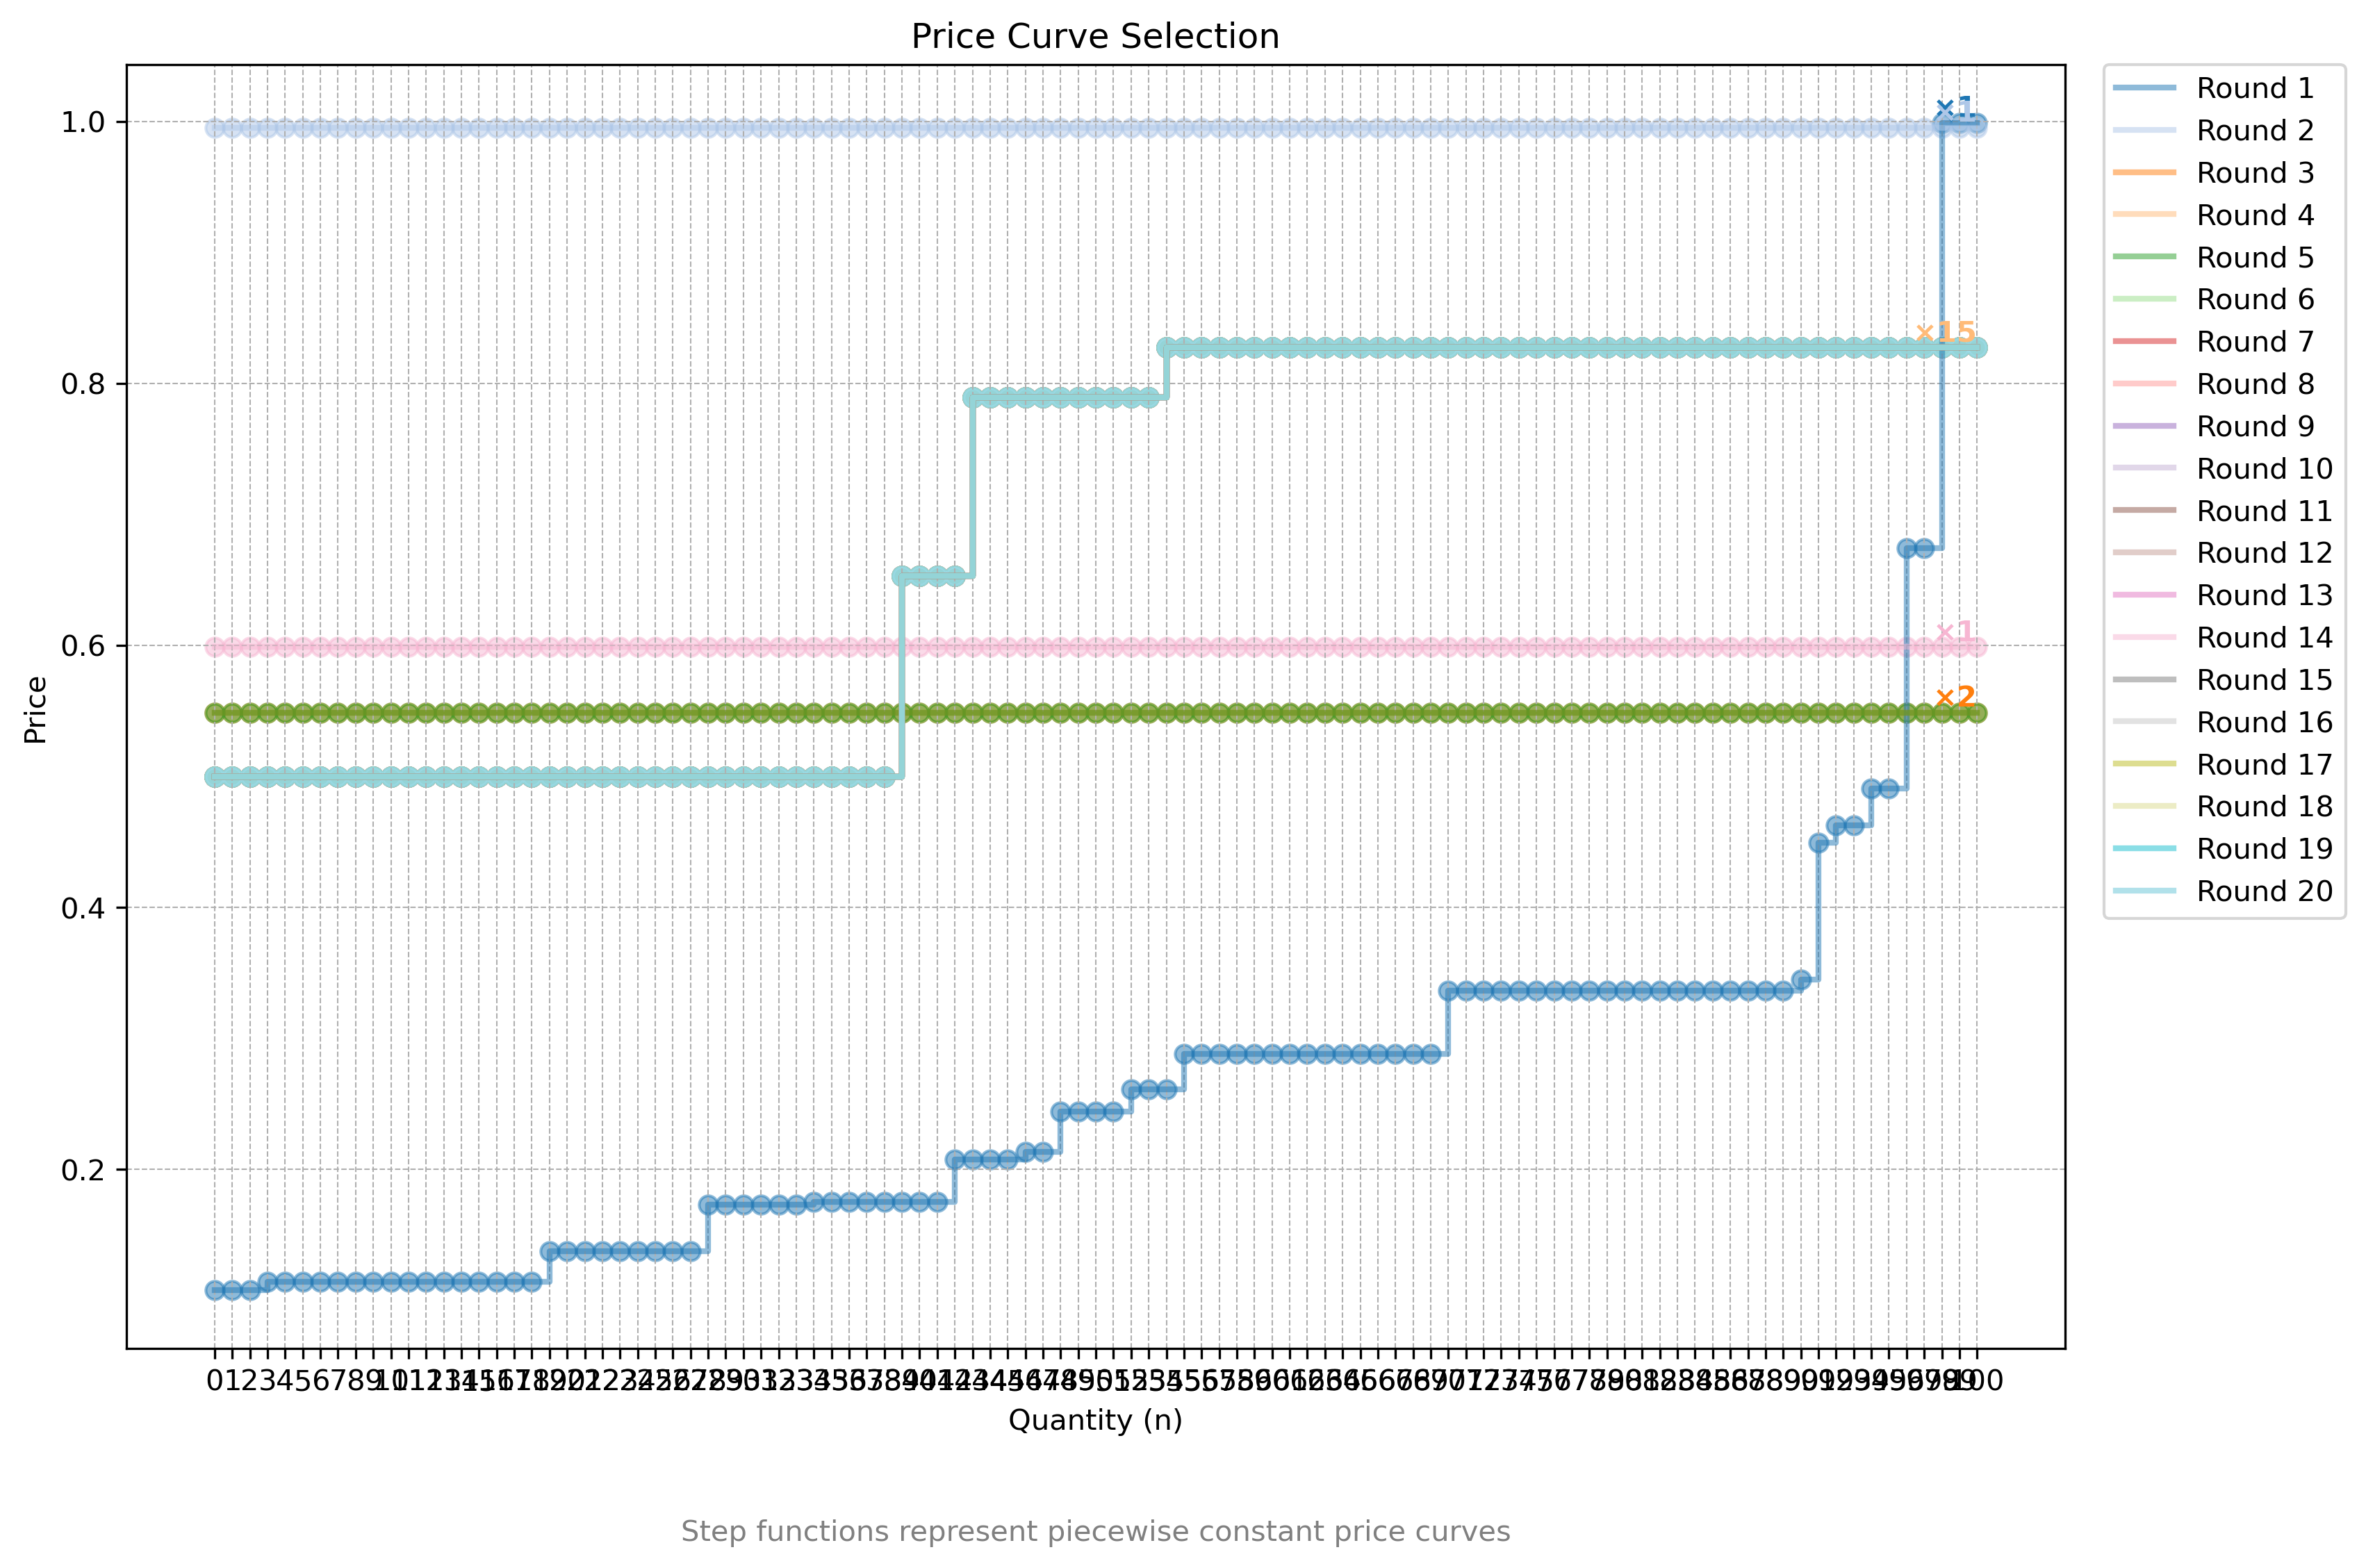
\includegraphics[width=0.92\textwidth]{figures/FTPL_price_curve_selection}
    \caption{FTPL 价格曲线选择情况}
\end{figure}

这里使用了折线图展示了所有的价格曲线的选择情况。横坐标为轮次,纵坐标为价格,标记了不同价格曲线的选择次数。

\begin{figure}[H]
    \centering
    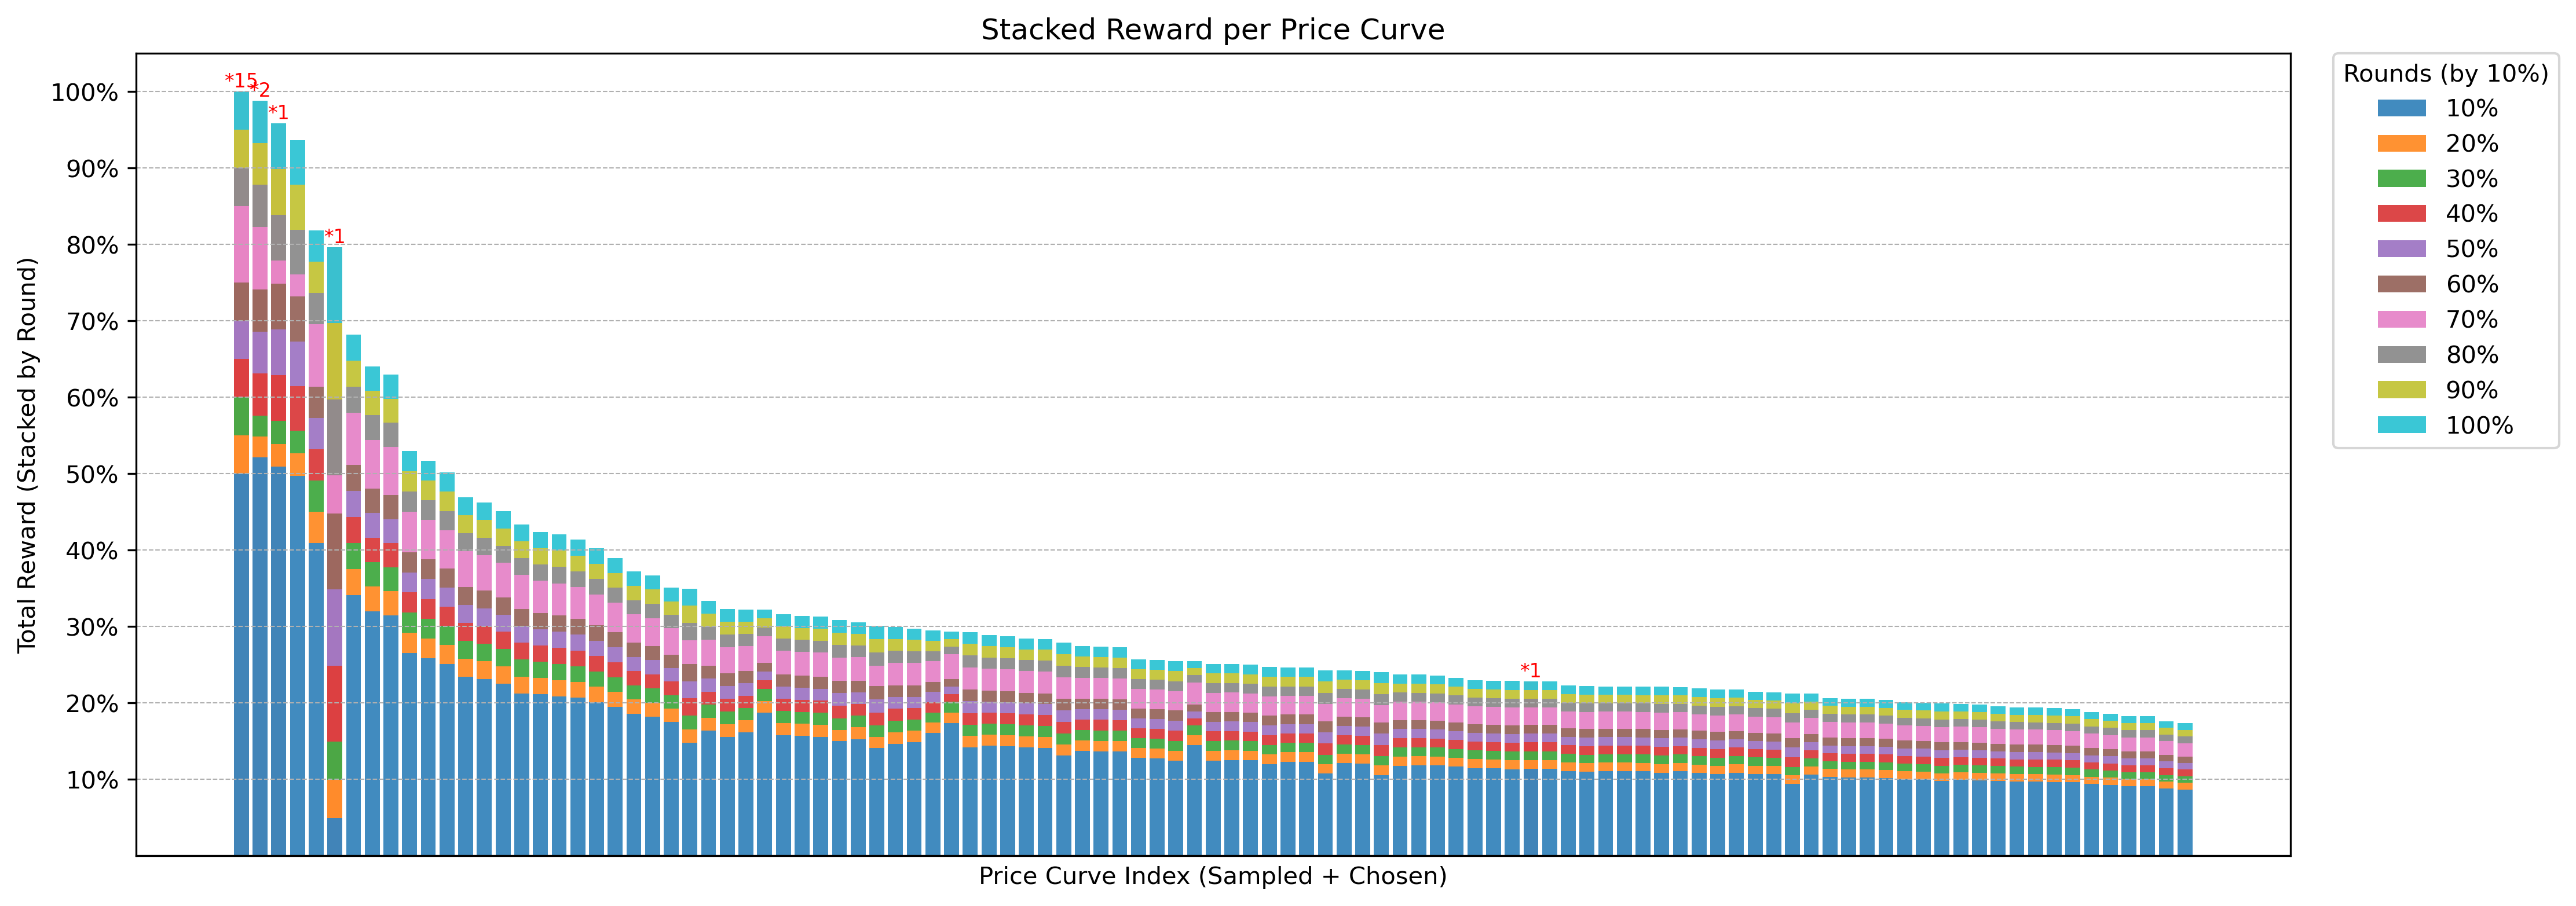
\includegraphics[width=0.92\textwidth]{figures/FTPL_reward_distribution}
    \caption{FTPL 奖励分布}
\end{figure}

这里展示了 FTPL 算法中每个价格曲线的奖励分布情况。横坐标为价格曲线的索引,纵坐标为对应的奖励值。为了方便显示,这里从所有价格曲线中随机选择了 100 条,并加上所有被选中的价格曲线进行展示;纵向按照轮数的 10\% 进行划分和累加。价格曲线按照总奖励值从大到小排序,用选中次数来标记被选中的价格曲线。

可以看到被选中的价格曲线的奖励都比较高,这正反映了 FTPL 算法的选择策略。

\begin{figure}[H]
    \centering
    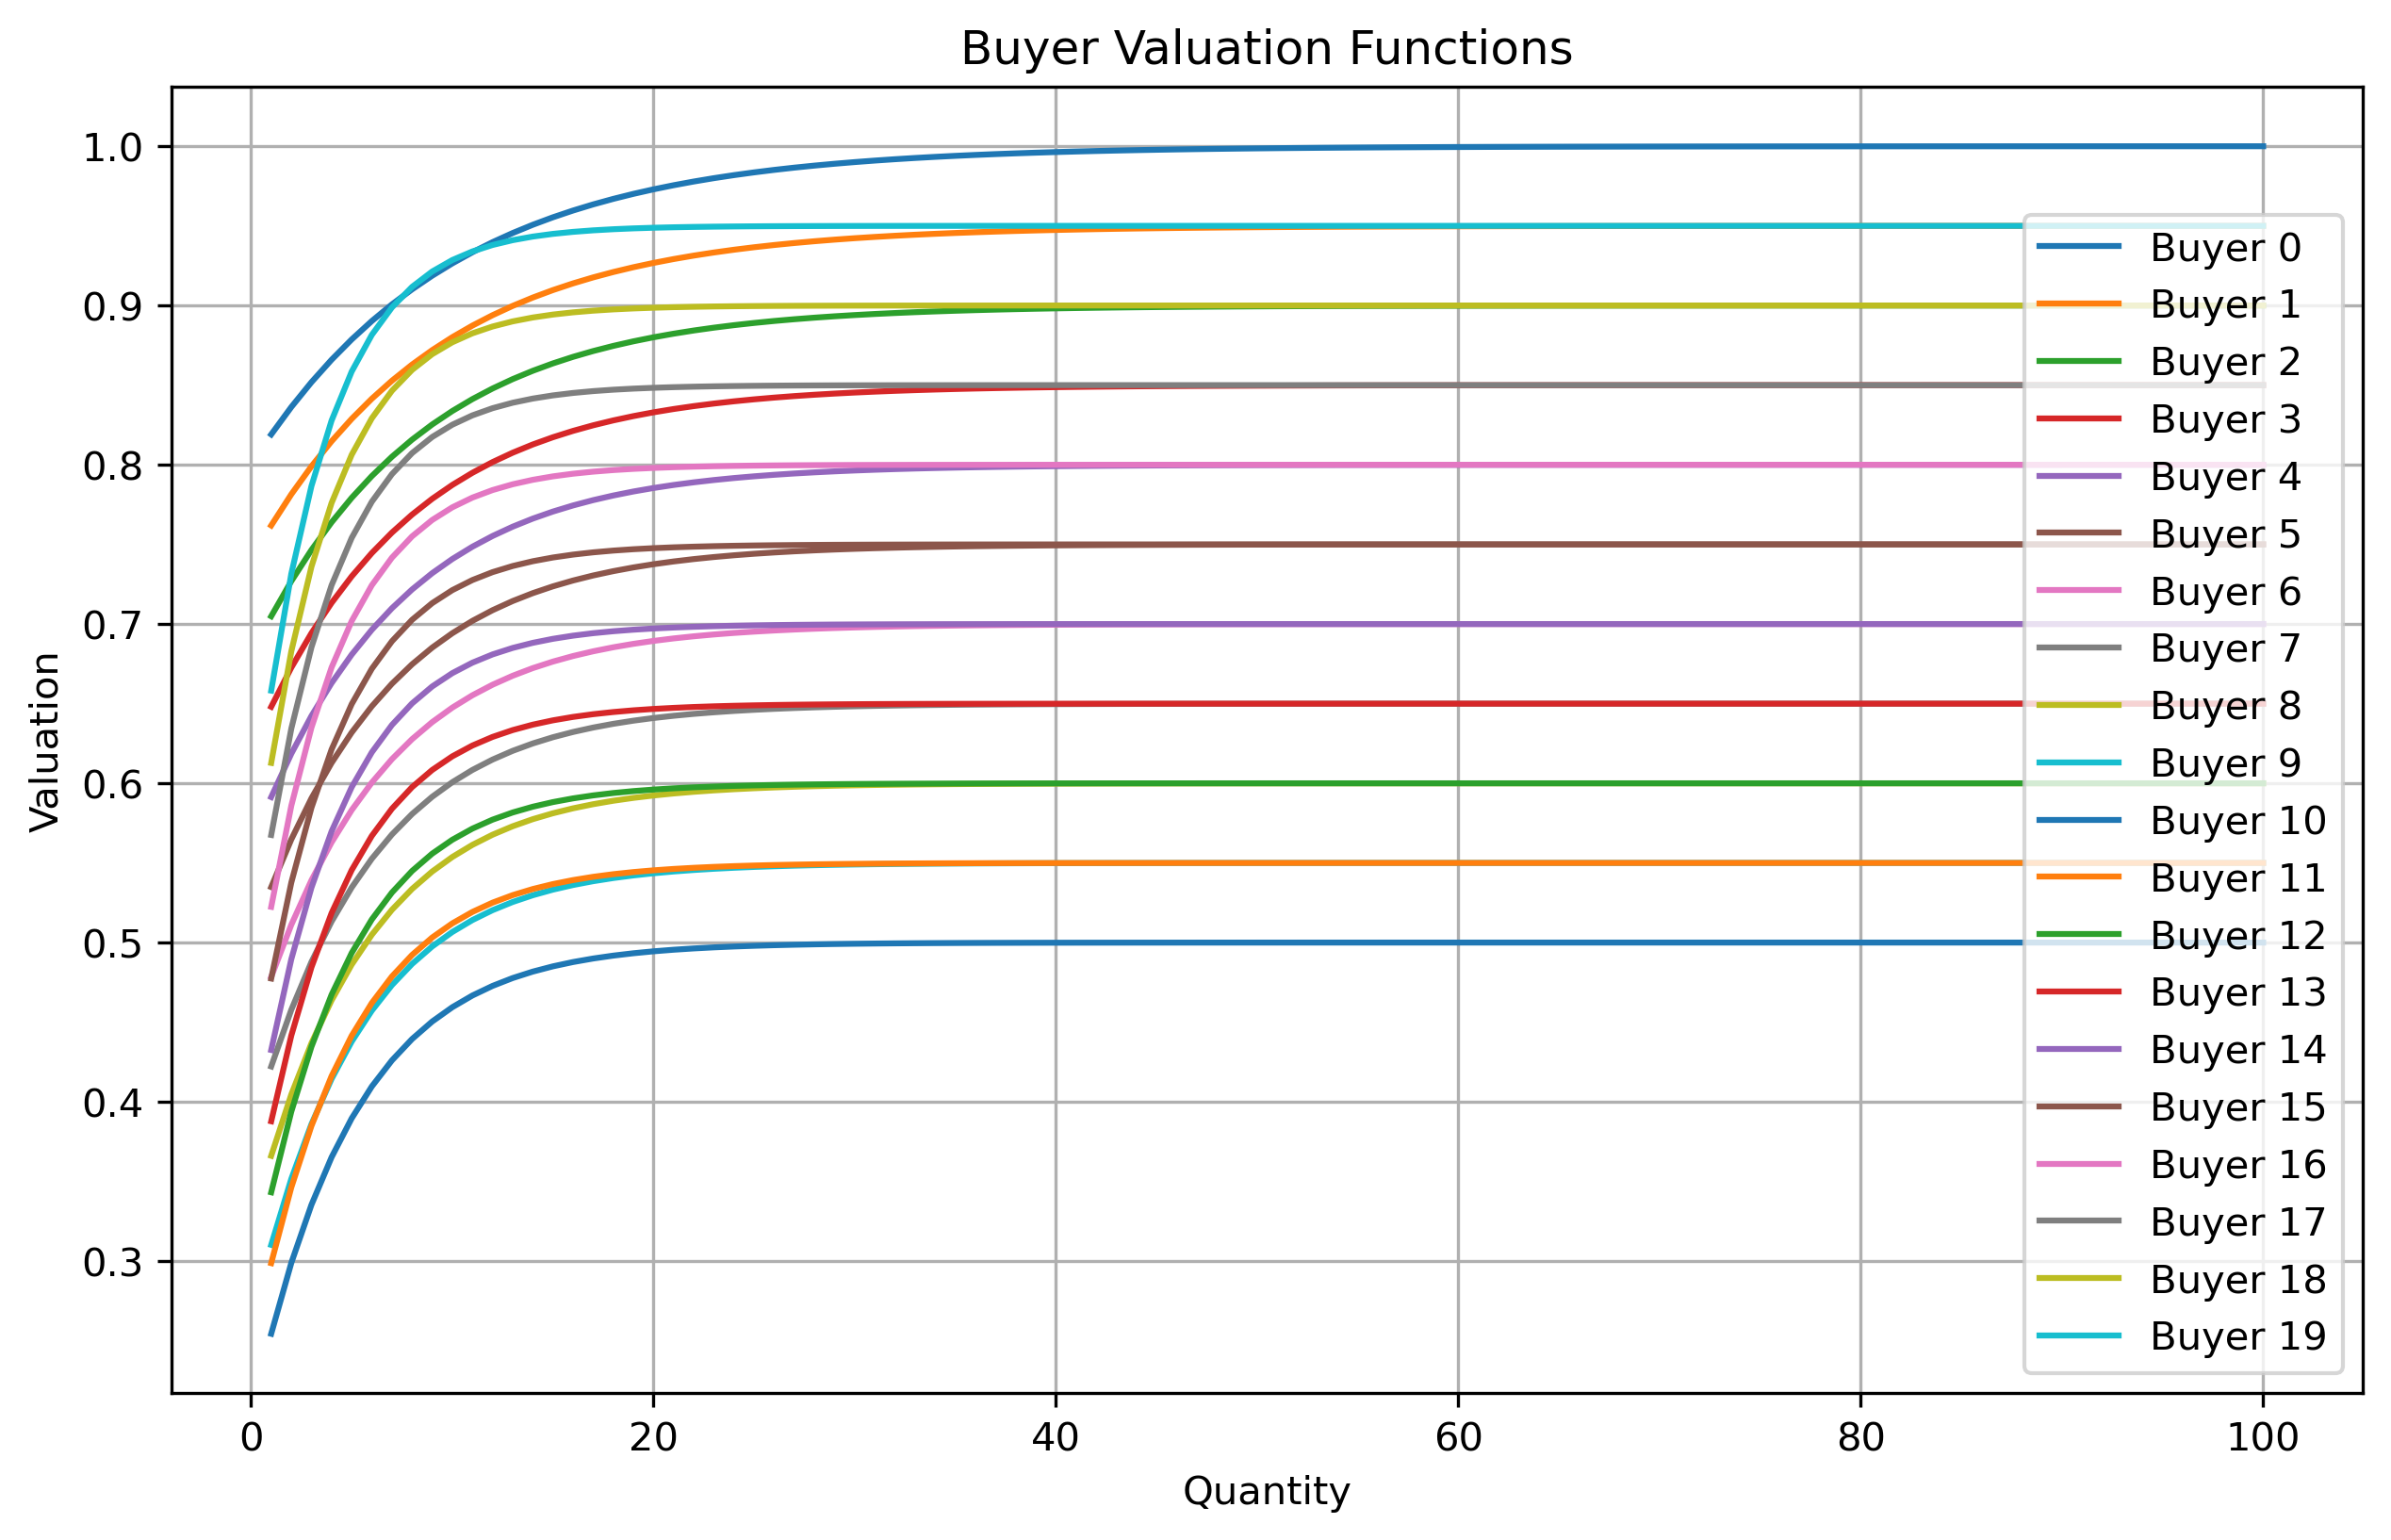
\includegraphics[width=0.92\textwidth]{figures/FTPL_valuation_functions}
    \caption{FTPL 买家估值函数}
\end{figure}

这里展示了 FTPL 算法中买家的估值函数。横坐标为物品数量,纵坐标为估值函数的值,不同颜色的曲线表示不同买家类型的估值函数。